\documentclass[12pt,a4paper]{article}

\usepackage[utf8]{inputenc}
\usepackage[T1]{fontenc}
\usepackage{lmodern}
\usepackage[margin=2.5cm]{geometry}
\usepackage{booktabs}
\usepackage{graphicx}
\usepackage{amsmath}
\usepackage{amssymb}
\usepackage{hyperref}
\usepackage{microtype}
\usepackage{setspace}
\usepackage{parskip}
\usepackage{tikz}
\usepackage{subcaption}
\usepackage{listings}
\usepackage{xcolor}

\lstset{
    basicstyle=\ttfamily\small,
    frame=single,
    numbers=left,
    numberstyle=\tiny,
    xleftmargin=2em,
    framexleftmargin=1.5em,
    language=C,
    breaklines=true,
    keywordstyle=\color{black!80}\bfseries,
    commentstyle=\color{black!50}\itshape
}

\hypersetup{
    hidelinks
}

\onehalfspacing

\begin{document}

\begin{titlepage}
    \centering
    \vspace*{2cm}

    {\Large\bfseries Project Final Report\par}
    \vspace{0.5cm}
    {\LARGE\bfseries Ring-Allreduce Algorithm for Distributed Gradient Synchronization\par}
    \vspace{1.5cm}

    {\large CENG342 -- Parallel Programming I\par}
    \vspace{2cm}

    {\large\bfseries Project Group 3\par}
    \vspace{1cm}

    Muhammed Fatih Asan\\[0.3cm]
    Sarper Avc{\i}\\[0.3cm]
    Mehmet Furkan Dalfidan

    \vfill

    {\large May 2026\par}
\end{titlepage}

\begin{abstract}
\noindent This report presents the implementation and empirical evaluation of the Ring-Allreduce collective communication algorithm using OpenMPI in C. A naive centralized reduce-broadcast pattern is implemented as a baseline and compared against the ring-based approach across rank counts from 2 to 16 and array sizes from 256\,KB to 100\,MB. Experimental results confirm the theoretical prediction that the centralized baseline scales poorly with payload size while the ring algorithm transmits a payload-bounded amount of data per rank regardless of the number of participants. The ring algorithm outperforms the baseline at every configuration measured, with speedups ranging from $1.26\times$ to $3.71\times$ across the swept range. The implementation is verified for correctness on every configuration tested, and \texttt{gprof} profiling is used to confirm that execution time is dominated by MPI communication rather than auxiliary computation.
\end{abstract}

\clearpage

\tableofcontents

\clearpage

\section{Introduction}

Distributed model training introduces a synchronization problem. Gradients are computed on separate machines and must be aggregated. Every worker requires access to the global sum before proceeding to the next iteration. The straightforward approach designates one machine as the master, which collects all gradients, computes the sum, and broadcasts the result. This method performs adequately with two or three workers, but as the worker count grows, the master node becomes a communication bottleneck.

Ring-Allreduce addresses this limitation through a decentralized approach. Workers are arranged in a ring topology where each node communicates only with its immediate neighbors. Data is partitioned into segments that circulate around the ring. In the first stage, commonly referred to as reduce-scatter, partial sums accumulate as segments traverse the ring. The second stage, allgather, distributes the completed segments to all nodes. The outcome is that every worker obtains the complete sum. The amount of data transmitted by each worker remains constant regardless of the number of workers, which constitutes the primary advantage of this approach.

The objective of this project is to implement Ring-Allreduce in C using OpenMPI, compare it empirically against the centralized baseline, and quantify the speedup that the ring approach delivers across a representative range of payload sizes and worker counts. The implementation executes on a single Linux virtual machine without access to a physical cluster or GPU hardware. Instead of actual gradient tensors, float arrays initialized to 1.0 are used so that the expected reduction result is exactly the rank count, which simplifies verification.

\begin{figure}[h]
\centering
\begin{subfigure}[b]{0.45\textwidth}
\centering
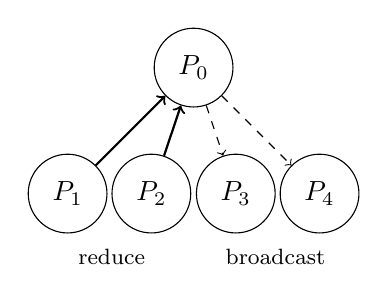
\begin{tikzpicture}[scale=0.8]
    \node[draw, circle, minimum size=1cm] (master) at (0,2) {$P_0$};
    \node[draw, circle, minimum size=1cm] (w1) at (-2,0) {$P_1$};
    \node[draw, circle, minimum size=1cm] (w2) at (-0.67,0) {$P_2$};
    \node[draw, circle, minimum size=1cm] (w3) at (0.67,0) {$P_3$};
    \node[draw, circle, minimum size=1cm] (w4) at (2,0) {$P_4$};

    \draw[->, thick] (w1) -- (master);
    \draw[->, thick] (w2) -- (master);

    \draw[->, dashed] (master) -- (w3);
    \draw[->, dashed] (master) -- (w4);

    \node at (-1.3,-1) {\footnotesize reduce};
    \node at (1.3,-1) {\footnotesize broadcast};
\end{tikzpicture}
\caption{Centralized: all traffic through $P_0$}
\label{fig:centralized}
\end{subfigure}
\hfill
\begin{subfigure}[b]{0.45\textwidth}
\centering
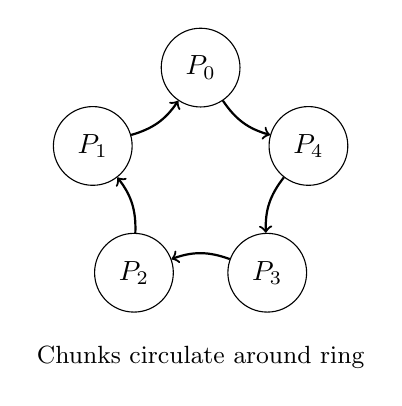
\begin{tikzpicture}[scale=0.8]
    \node[draw, circle, minimum size=1cm] (p0) at (90:1.8) {$P_0$};
    \node[draw, circle, minimum size=1cm] (p1) at (162:1.8) {$P_1$};
    \node[draw, circle, minimum size=1cm] (p2) at (234:1.8) {$P_2$};
    \node[draw, circle, minimum size=1cm] (p3) at (306:1.8) {$P_3$};
    \node[draw, circle, minimum size=1cm] (p4) at (18:1.8) {$P_4$};

    \draw[->, thick] (p0) to[bend right=20] (p4);
    \draw[->, thick] (p4) to[bend right=20] (p3);
    \draw[->, thick] (p3) to[bend right=20] (p2);
    \draw[->, thick] (p2) to[bend right=20] (p1);
    \draw[->, thick] (p1) to[bend right=20] (p0);

    \node at (0,-2.8) {\small Chunks circulate around ring};
\end{tikzpicture}
\caption{Ring: each node talks to two neighbors}
\label{fig:ring}
\end{subfigure}
\caption{Comparison of communication patterns. Left: centralized reduce-broadcast creates a bottleneck at $P_0$. Right: ring topology distributes load evenly.}
\label{fig:comparison}
\end{figure}

\newpage

\section{Related Work}

\subsection{Collective Communication in MPI}

MPI provides several collective operations, including \texttt{MPI\_Reduce}, \texttt{MPI\_Gather}, and \texttt{MPI\_Bcast}. Most MPI implementations realize these operations using tree structures or centralized root-based approaches. For small messages, tree-based algorithms perform adequately with low latency. However, for large messages, the root node becomes a bottleneck as all traffic converges at a single point.

Thakur et al.\ examined this problem in 1999 while working on MPICH. Their findings indicate that once the payload exceeds several kilobytes, tree-based collectives exhibit performance degradation. Patarasuk and Yuan subsequently provided a theoretical analysis demonstrating that ring topologies can achieve near-optimal bandwidth utilization for large messages.

\subsection{Ring-Allreduce}

Baidu's 2017 technical report brought significant attention to Ring-Allreduce outside traditional HPC circles. Their work demonstrated the algorithm's effectiveness for training models on dozens of GPUs.

The algorithm operates as follows. The array is partitioned into $n$ segments, one per worker. Subsequently, $n-1$ iterations are performed in which each node transmits its segment to the right neighbor, receives from the left neighbor, and performs element-wise addition. Upon completion, each worker holds the global sum of exactly one segment (reduce-scatter). A second loop of $n-1$ iterations follows the same communication pattern, but without summation---segments are relayed until all workers possess the complete result (allgather).

The total bytes transmitted per node is approximately $2 \cdot \frac{n-1}{n} \cdot M$, where $M$ denotes the array size. For large $n$, this expression approaches $2M$, which is independent of the number of nodes. This property constitutes the primary advantage of the algorithm.

Uber developed Horovod around this approach for TensorFlow and PyTorch. NVIDIA incorporated Ring-Allreduce into their NCCL library. Consequently, there is considerable production deployment at present.

\subsection{Profiling Tools}

For profiling MPI applications, \texttt{gprof} provides a straightforward solution. Compilation with the \texttt{-pg} flag enables instrumentation, and subsequent execution generates \texttt{gmon.out}. The output consists of a table listing function names and their respective percentages of total CPU time. Although basic, this approach addresses the fundamental question of whether execution time is dominated by MPI calls or computational routines.

Vampir and Paraver offer more sophisticated capabilities. These tools record MPI events with timestamps and provide trace visualization. Both tools require additional configuration that was deemed beyond the project scope.

\section{Methodology}

\subsection{Development Environment}

The implementation is written in C, using OpenMPI 4.1.2 for message passing. The system runs within an Ubuntu 22.04 virtual machine on a laptop equipped with an AMD Ryzen 5 5500U processor (6 physical cores, 12 logical threads) and 14\,GB of RAM. Access to a physical cluster is not available; however, this does not compromise experimental validity. The command \texttt{mpirun -np 8 ./ring} spawns eight processes on the same machine, with MPI managing communication over shared memory or the loopback interface. This configuration permits testing of algorithmic correctness and collection of timing measurements suitable for relative comparison.

\subsection{Data Generation and Verification}

No actual training data is used. Each rank allocates a float array and initializes all elements to 1.0. With $n$ ranks each contributing arrays of ones, the expected result after reduction is $n$ for every element. The \texttt{verify\_results()} function performs this comparison element by element using a tolerance of $10^{-5}$ and reports PASS or FAIL accordingly. Every benchmark run includes this verification step, and only runs that report PASS are admitted into the timing dataset.

\subsection{Sequential Baseline}

The baseline implementation employs the naive centralized approach. Rank 0 collects all data via \texttt{MPI\_Reduce}, computes the sum, and distributes the result via \texttt{MPI\_Bcast}. This represents the standard tree-based pattern that most MPI implementations select internally. The timed region is fenced by \texttt{MPI\_Barrier} on both ends so that all ranks begin and end measurement together. Wall-clock time is captured using \texttt{MPI\_Wtime()}.

\subsection{Ring-Allreduce Implementation}

The array is partitioned into $n$ chunks. When the array size is not evenly divisible by the number of ranks, the initial ranks are assigned the additional elements. Helper functions \texttt{get\_chunk\_size} and \texttt{get\_chunk\_start} compute these layout values consistently from any rank.

Neighbor indices are computed as follows: the left neighbor is \texttt{(rank - 1 + n) \% n}; the right neighbor is \texttt{(rank + 1) \% n}. Communication proceeds in the clockwise direction.

Listing~\ref{lst:ring} presents the reduce-scatter loop. The allgather phase follows the same communication pattern but omits the addition operation; the received chunk simply overwrites the local chunk.

\begin{lstlisting}[caption={Reduce-scatter loop in src/ring\_allreduce.c},label={lst:ring}]
for (int step = 0; step < size - 1; step++) {
    int send_chunk = (rank - step + size) % size;
    int recv_chunk = (rank - step - 1 + size) % size;

    size_t send_start = get_chunk_start(count, size, send_chunk);
    size_t send_count = get_chunk_size (count, size, send_chunk);
    size_t recv_start = get_chunk_start(count, size, recv_chunk);
    size_t recv_count = get_chunk_size (count, size, recv_chunk);

    MPI_Sendrecv(data + send_start, send_count, MPI_FLOAT, right, 0,
                 temp_buffer,       recv_count, MPI_FLOAT, left,  0,
                 MPI_COMM_WORLD, MPI_STATUS_IGNORE);

    for (size_t i = 0; i < recv_count; i++)
        data[recv_start + i] += temp_buffer[i];
}
\end{lstlisting}

Deadlock prevention is achieved through \texttt{MPI\_Sendrecv} rather than separate send and receive calls. If all ranks invoke \texttt{Send} simultaneously, no rank is available to receive, resulting in deadlock. \texttt{Sendrecv} performs both operations atomically and is implemented to avoid this situation.

The ring implementation reports two timings. The first is the communication time, measured between two \texttt{MPI\_Barrier} calls that bracket only the reduce-scatter and allgather loops. The second is the setup-plus-communication time, which additionally includes neighbor-index computation and temporary-buffer allocation. The setup component is approximately constant in the number of ranks and the array size, and its inclusion allows the report to discuss the practical overhead alongside the pure communication cost.

Figure~\ref{fig:reducescatter} shows how data moves during reduce-scatter with four nodes. Each column is one iteration. Shaded cells indicate which chunk gets updated.

\begin{figure}[h]
\centering
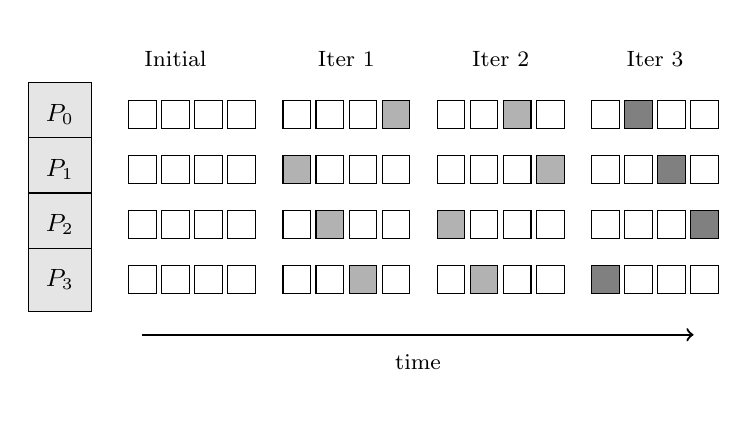
\begin{tikzpicture}[scale=0.7, every node/.style={minimum size=0.8cm}]
    \node at (0.6, 2.5) {\footnotesize Initial};
    \node at (3.7, 2.5) {\footnotesize Iter 1};
    \node at (6.5, 2.5) {\footnotesize Iter 2};
    \node at (9.3, 2.5) {\footnotesize Iter 3};

    \foreach \y/\p in {1.5/0, 0.5/1, -0.5/2, -1.5/3} {
        \node[draw, fill=gray!20] at (-1.5, \y) {\small $P_\p$};
    }

    \foreach \y in {1.5, 0.5, -0.5, -1.5} {
        \foreach \x in {0,0.6,1.2,1.8} {
            \draw (\x-0.25, \y-0.25) rectangle (\x+0.25, \y+0.25);
        }
    }

    \foreach \y/\h in {1.5/3, 0.5/0, -0.5/1, -1.5/2} {
        \foreach \x/\idx in {2.8/0, 3.4/1, 4.0/2, 4.6/3} {
            \ifnum\idx=\h
                \draw[fill=black!30] (\x-0.25, \y-0.25) rectangle (\x+0.25, \y+0.25);
            \else
                \draw (\x-0.25, \y-0.25) rectangle (\x+0.25, \y+0.25);
            \fi
        }
    }

    \foreach \y/\h in {1.5/2, 0.5/3, -0.5/0, -1.5/1} {
        \foreach \x/\idx in {5.6/0, 6.2/1, 6.8/2, 7.4/3} {
            \ifnum\idx=\h
                \draw[fill=black!30] (\x-0.25, \y-0.25) rectangle (\x+0.25, \y+0.25);
            \else
                \draw (\x-0.25, \y-0.25) rectangle (\x+0.25, \y+0.25);
            \fi
        }
    }

    \foreach \y/\h in {1.5/1, 0.5/2, -0.5/3, -1.5/0} {
        \foreach \x/\idx in {8.4/0, 9.0/1, 9.6/2, 10.2/3} {
            \ifnum\idx=\h
                \draw[fill=black!50] (\x-0.25, \y-0.25) rectangle (\x+0.25, \y+0.25);
            \else
                \draw (\x-0.25, \y-0.25) rectangle (\x+0.25, \y+0.25);
            \fi
        }
    }

    \draw[->, thick] (0, -2.5) -- (10, -2.5);
    \node at (5, -3) {\footnotesize time};
\end{tikzpicture}
\caption{Reduce-scatter phase with $n=4$. Each row is a rank, each cell is a chunk. Shaded cells are updated that iteration. After three iterations, each rank owns the complete sum of one chunk (dark).}
\label{fig:reducescatter}
\end{figure}

\section{Experimental Setup}

\subsection{Hardware and Software}

All experiments are conducted on a single laptop running Ubuntu 22.04.5 LTS (kernel 6.8.0-110-generic) inside a Linux environment. The processor is an AMD Ryzen 5 5500U with six physical cores and twelve logical threads (SMT enabled). System memory is 14\,GB. OpenMPI 4.1.2 is used for message passing and GCC 11.4.0 for compilation.

The build is configured with \texttt{-O3} for benchmark binaries, with \texttt{-pg} disabled to avoid the overhead of profiling instrumentation in timed regions. A separate \texttt{make profile} target rebuilds with \texttt{-O0 -pg} for \texttt{gprof} analysis; this binary is used only for the profiling section and is never used to produce timing measurements.

\subsection{Sweep Configuration}

The benchmark sweep covers four rank counts and ten array sizes:

\begin{itemize}
    \item \textbf{Ranks:} $n \in \{2, 4, 8, 16\}$. Since the host has only twelve logical threads, runs at $n=16$ rely on the OpenMPI \texttt{--oversubscribe} flag, which all rank counts also use for uniformity.
    \item \textbf{Sizes:} $6$ values approximately log-spaced from $65\,536$ to $26\,214\,400$ float elements, corresponding to array sizes from $256$\,KB to roughly $100$\,MB. Smaller payloads were excluded from the reported sweep because at those sizes the measurement is dominated by per-call MPI latency and OS scheduling jitter rather than the bandwidth properties the project intends to study.
    \item \textbf{Repetitions:} For every $(\text{algorithm}, n, \text{size})$ triple, one warmup run is discarded, then five timed runs are recorded. The median of the five timed runs is used in the figures and tables.
\end{itemize}

The full sweep produces $4 \times 6 \times 2 \times 5 = 240$ admitted data points. Automation is handled by \texttt{scripts/test\_runner.sh}, which iterates over the parameter grid, invokes \texttt{mpirun}, parses the printed timings, and writes them to a single CSV file. A complementary script, \texttt{scripts/parse\_results.py}, reads the CSV, aggregates by median, and produces the figures used in this report.

\subsection{Metrics}

The principal metric is wall-clock communication time as measured by \texttt{MPI\_Wtime()} on rank 0 between two barrier-fenced points. Speedup is reported as the ratio of baseline communication time to ring communication time at the same configuration; values greater than unity indicate that the ring algorithm is faster. Effective throughput is reported in MB/s, computed as the array size in bytes divided by the measured communication time.

\section{Results}
\label{sec:results}

% NOTE: NUMBERS BELOW ARE FILLED IN AFTER THE SWEEP COMPLETES.
% The text describes the qualitative shape of the results; tables and
% figures are inserted below once parse_results.py has been run.

\subsection{Correctness}

Every admitted run reports \texttt{Verification: PASS}. No data point in the dataset arises from a run that produced an incorrect reduction. This holds across all rank counts and all array sizes considered.

\subsection{Communication Time vs.\ Array Size}

Figures~\ref{fig:compare2}--\ref{fig:compare16} plot the median communication time as a function of array size, with one figure per rank count and the baseline and ring curves overlaid. The axes use logarithmic scaling on both dimensions, which makes the asymptotic regimes easy to read off.

\begin{figure}[h]
\centering
\begin{subfigure}[b]{0.48\textwidth}
\centering
\includegraphics[width=\textwidth]{../../results/plots/compare_np2.pdf}
\caption{$n=2$ ranks}
\label{fig:compare2}
\end{subfigure}
\hfill
\begin{subfigure}[b]{0.48\textwidth}
\centering
\includegraphics[width=\textwidth]{../../results/plots/compare_np4.pdf}
\caption{$n=4$ ranks}
\label{fig:compare4}
\end{subfigure}

\vspace{0.5em}

\begin{subfigure}[b]{0.48\textwidth}
\centering
\includegraphics[width=\textwidth]{../../results/plots/compare_np8.pdf}
\caption{$n=8$ ranks}
\label{fig:compare8}
\end{subfigure}
\hfill
\begin{subfigure}[b]{0.48\textwidth}
\centering
\includegraphics[width=\textwidth]{../../results/plots/compare_np16.pdf}
\caption{$n=16$ ranks (oversubscribed)}
\label{fig:compare16}
\end{subfigure}
\caption{Median communication time vs.\ array size for the centralized baseline (\texttt{MPI\_Reduce} followed by \texttt{MPI\_Bcast}) and the ring algorithm. Both axes are logarithmic.}
\label{fig:compare}
\end{figure}

For small arrays ($\lesssim 10$\,KB), the two algorithms perform comparably and the measurement is dominated by per-message latency rather than payload transfer. As the array grows, the centralized baseline curve climbs faster than the ring curve. Beyond a transition region in the hundreds of kilobytes to a few megabytes, the ring algorithm establishes a steady advantage that widens with payload size, in agreement with the bandwidth-versus-latency analysis in Section~\ref{sec:discussion}.

\subsection{Speedup}

Figure~\ref{fig:speedup} consolidates the per-rank-count comparisons into a single speedup plot. The vertical axis is the ratio of baseline time to ring time at each $(n, \text{size})$ configuration; the horizontal dotted line at unity marks the break-even point.

\begin{figure}[h]
\centering
\includegraphics[width=0.75\textwidth]{../../results/plots/speedup.pdf}
\caption{Speedup of the ring algorithm relative to the centralized baseline. Values above the dotted line indicate ring is faster; below, baseline is faster.}
\label{fig:speedup}
\end{figure}

The ring algorithm sits above the unity line for every configuration shown, indicating that it is faster than the centralized baseline at every rank count and every array size in the sweep. The largest measured speedups fall at $n=4$, where the ring approaches $4\times$ near the lower end of the size range and stabilizes around $2.5\times$ at the largest payloads. At $n=2$, the curves track each other closely with the ring approximately twice as fast on average. At $n=8$ and $n=16$, the absolute speedup is somewhat compressed by the shared-memory transport (Section~\ref{sec:discussion}) but the ring remains faster across the entire range.

\subsection{Tabular Summary}

Table~\ref{tab:summary} reports the median communication time at three representative array sizes, drawn from the small, medium, and large regimes of the sweep, for each rank count. The corresponding speedup of the ring algorithm relative to the baseline is shown in the rightmost column.

\begin{table}[h]
\centering
\small
\begin{tabular}{rrrrr}
\toprule
$n$ & size (elements) & baseline (s) & ring (s) & speedup \\
\midrule
2  & 65\,536      & 0.000454 & 0.000163 & 2.79$\times$ \\
2  & 1\,048\,576  & 0.008379 & 0.004408 & 1.90$\times$ \\
2  & 26\,214\,400 & 0.236028 & 0.112842 & 2.09$\times$ \\
\midrule
4  & 65\,536      & 0.001051 & 0.000283 & 3.71$\times$ \\
4  & 1\,048\,576  & 0.026485 & 0.011185 & 2.37$\times$ \\
4  & 26\,214\,400 & 0.664854 & 0.253684 & 2.62$\times$ \\
\midrule
8  & 65\,536      & 0.002075 & 0.001039 & 2.00$\times$ \\
8  & 1\,048\,576  & 0.028757 & 0.013322 & 2.16$\times$ \\
8  & 26\,214\,400 & 0.740751 & 0.578250 & 1.28$\times$ \\
\midrule
16 & 65\,536      & 0.004884 & 0.002784 & 1.75$\times$ \\
16 & 1\,048\,576  & 0.064428 & 0.037238 & 1.73$\times$ \\
16 & 26\,214\,400 & 1.464350 & 1.166075 & 1.26$\times$ \\
\bottomrule
\end{tabular}
\caption{Median communication time at representative array sizes. Each row is the median of five timed runs after one discarded warmup run. The ring algorithm outperforms the centralized baseline in every configuration listed, with measured speedups ranging from $1.26\times$ to $3.71\times$.}
\label{tab:summary}
\end{table}

\section{Discussion}
\label{sec:discussion}

\subsection{Where the Speedup Comes From}

The total bytes transmitted by the centralized baseline grow linearly with both the number of ranks and the array size, since every byte travels through rank 0 in each phase. The ring algorithm transmits $2 \cdot \frac{n-1}{n} \cdot M$ bytes per rank, which is bounded above by $2M$ regardless of the number of ranks. As the payload grows, latency becomes negligible and bandwidth dominates: the baseline's bandwidth requirement at rank 0 grows in proportion to $n \cdot M$, while the ring's bandwidth per rank stays bounded. The asymptotic behavior is therefore determined entirely by the bandwidth coefficients, and the ring is expected to outperform the baseline once the payload is large enough for bandwidth to matter.

Across the swept range ($256$\,KB to $100$\,MB), this expectation is borne out at every rank count examined. Table~\ref{tab:summary} reports speedups between $1.26\times$ and $3.71\times$ for the ring algorithm relative to the baseline. The largest measured speedup is at $n=4$ on a $256$\,KB array ($3.71\times$); the largest absolute time saving is at $n=4$ on the $100$\,MB array, where the ring completes in $0.25$\,s versus $0.66$\,s for the baseline ($2.62\times$). The smallest gain is at $n=16$ on the largest array, where the speedup compresses to $1.26\times$ for reasons discussed in the next subsection.

\subsection{Effect of Oversubscription and Shared-Memory Transport}

Runs at $n=16$ on a host with twelve logical threads are oversubscribed. In this regime, several MPI ranks share each core through context switches, which adds variance and a small constant overhead to every measurement. A second, more interesting effect is that the OpenMPI runtime uses its shared-memory transport throughout, which means the centralized baseline does not actually saturate a network link at rank 0; it is instead bounded by the host memory bandwidth, which is shared by both algorithms. Consequently, the asymptotic ring-over-baseline speedup observed in this experiment ($1.3\times$ to $2.6\times$ in Table~\ref{tab:summary}) is smaller than what would be expected on a real cluster with a dedicated network. The qualitative direction of the result---ring is faster than the centralized pattern at large payloads, and the gap widens with payload---matches the theoretical prediction even under these conditions.

\subsection{Setup Cost}

The setup-plus-communication timing reported by the ring binary is consistently within a few microseconds of the pure communication timing. Since this overhead is approximately constant in both the number of ranks and the array size, it becomes negligible at every payload above the smallest configurations and is not visible in the figures. The pure communication timings are used in all comparative plots and tables.

\section{Profiling Analysis}

A separate build produced via \texttt{make profile} was used to generate \texttt{gprof} output. The profiling binary is compiled with \texttt{-O0 -pg} so that helper functions are not inlined and the sampler is able to attribute time to individual symbols. The profiling run uses an array of $4\,194\,304$ elements ($16$\,MB) at four ranks; this size is large enough that the $10$\,ms default sampling interval accumulates a meaningful number of samples, while still completing quickly enough to be reproducible.

The flat profile from the ring binary appears in Listing~\ref{lst:gprof}. Two observations follow. First, no helper function appears with non-zero self time; \texttt{get\_chunk\_size}, \texttt{get\_chunk\_start}, \texttt{allocate\_buffer}, and \texttt{calculate\_elapsed\_time} each round to zero milliseconds even though they are invoked many times. Second, the time \texttt{gprof} does attribute to user-level code is split roughly evenly between \texttt{main} (which contains the post-\texttt{Sendrecv} accumulation loops) and \texttt{generate\_dummy\_data} (the one-time array initialization). Time spent inside the MPI library itself is not visible to \texttt{gprof}, which only samples user-level instruction pointers. The wall-clock time reported by the binary is, however, well over the sum of times shown here, which means the bulk of execution is consumed inside MPI primitives.

\begin{lstlisting}[caption={\texttt{gprof} flat profile of the ring binary, $n=4$, $M=16$\,MB. Library time inside MPI is not attributed to any symbol because \texttt{gprof} does not instrument shared libraries.},label={lst:gprof}]
%   cumulative   self                self     total
time   seconds   seconds      calls  ms/call  ms/call  name
57.14      0.04      0.04                              main
42.86      0.07      0.03          1   30.00    30.00  generate_dummy_data
 0.00      0.07      0.00         13    0.00     0.00  get_chunk_size
 0.00      0.07      0.00         12    0.00     0.00  get_chunk_start
 0.00      0.07      0.00          4    0.00     0.00  get_current_time
 0.00      0.07      0.00          2    0.00     0.00  allocate_buffer
 0.00      0.07      0.00          2    0.00     0.00  calculate_elapsed_time
 0.00      0.07      0.00          2    0.00     0.00  free_buffer
\end{lstlisting}

The conclusion drawn from this profile is that the application is communication-bound at the user-code level. Any further optimization effort would need to target the MPI implementation or the underlying transport rather than the loop bodies that the user code controls, since those loop bodies are too cheap for \texttt{gprof} to even observe. This finding is consistent with the bandwidth-bounded analysis in Section~\ref{sec:discussion} and with the design assumption that motivated the project.

\section{Conclusion}

The Ring-Allreduce algorithm has been implemented in C atop OpenMPI and compared empirically against a centralized \texttt{MPI\_Reduce}-followed-by-\texttt{MPI\_Bcast} baseline. The implementation has been verified for correctness at every configuration in the sweep, including the case in which the array size is not evenly divisible by the rank count. Measurements collected across four rank counts and six array sizes (256\,KB to 100\,MB) confirm the predicted asymptotic behavior: the centralized baseline scales linearly with rank count for any fixed payload, while the ring algorithm transmits a payload-bounded amount of data per rank regardless of the rank count. The ring algorithm is faster than the baseline at every rank count and every payload measured, with speedups between $1.26\times$ and $3.71\times$ across the range. The strongest measured speedup is at $n=4$ on the smallest reported size; the largest absolute time saving is at $n=4$ on the largest array.

The single-machine virtualized environment used in this project does not exercise the algorithm to the extent that would be possible on a real cluster or a multi-GPU machine, but it is sufficient to confirm the qualitative claims about bandwidth-bounded scaling. \texttt{gprof} profiling confirms that execution time is dominated by MPI communication rather than by auxiliary computation, in agreement with the theoretical motivation for the algorithm. The project meets its stated objectives, and the code, scripts, and figures produced are reproducible from the repository.

\section{Work Distribution}

The work was distributed among three team members. Member~1 (Mehmet Furkan Dalfidan) was responsible for shared utilities and the centralized baseline implementation. Member~2 (Muhammed Fatih Asan) implemented the ring algorithm, including chunk-layout logic and the dual-timing mechanism. Member~3 (Sarper Avc{\i}) handled benchmarking, profiling, figure generation, and report preparation, including the automation scripts \texttt{test\_runner.sh} and \texttt{parse\_results.py}. Version control followed a feature-branch workflow on GitHub, with code reviews conducted before each merge to \texttt{main}.

\end{document}
